The capacity spectrum method (CSM) was initially proposed by \citep{FreemanEtAl1975}, and it represents a simplified methodology for many purposes such as the evaluation of a large inventory of buildings, structural assessment of new or existing buildings or to identify the correlation between damage states and levels of ground motion. \cite{ATC1996} proposes three different procedures (A, B and C) for the application of the Capacity Spectrum Method. However, procedure B adopts some simplifications that might not always be valid and procedure C has a very strong graphical component, making it difficult for systematic applications. Hence, procedure A, which is characterized by its intuitiveness and simplicity, has been implemented in the RMTK.\\

This procedure iteratively compares the capacity and the demand of a structure, using a capacity curve (for the equivalent SDOF) and a damped response spectrum, respectively. The ground motion spectrum is computed for a level of equivalent viscous damping that is estimated as a function of the displacement at which the response spectrum crosses the capacity curve, in order to take into account the inelastic behaviour of the structure. Iterations are needed until there is a match between the equivalent viscous damping of the structure and the damping applied to the spectrum. The final intersection of these two curves approximates the target displacement response of the structure. This result is presented in Figure \ref{fig:per_point} for a "weak" and a "strong" ground motion record. \\

\begin{figure}[htb]
  \centering
      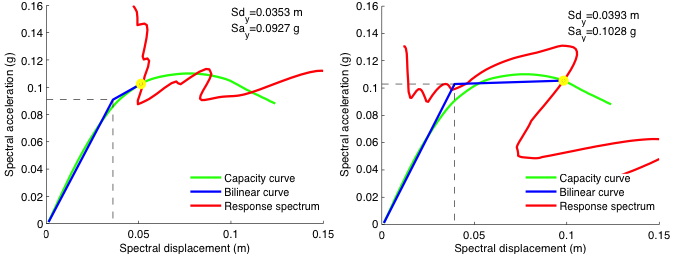
\includegraphics[width=12cm]{Figures/performance_points.png}
  \caption{Assessment of the target displacement for "weak" (left) and "strong" (strong) ground motion record.}
  \label{fig:per_point}
\end{figure}

The initial proposal of this method was heavily criticized due to its tendency to underestimate the deformation of the structures, which was mostly related with the model employed to calculate the equivalent viscous damping (e.g. \cite{Fajfar1999}; \cite{ChopraGoel2010}). Thus, in \cite{FEMA4402005}, some modifications were proposed regarding the calculation of this component. Furthermore, several other models relating an equivalent viscous damping with a ductility level have been proposed in the last decades, and implemented in the RMTK. The following list describes these models, and specifies the code that should be defined in the variable \verb=damping_model= in order to follow the assocuated model in the vulnerability calculations.\\

\begin{itemize}
\item \citep{FEMA4402005}:.
\item \citep{Kowalsky1994}:.
\item \citep{Iwan1980}:.
\item \citep{GulkanSozen1974}:.
\item \citep{PriesleyEtAl2007}:.
\item Masonry structures:.\\

\end{itemize}

This performance point is equivalent to what would be obtained by subjecting the equivalent single degree of freedom to a nonlinear time history analysis. This response (i.e. performance point) can be used to allocate the structure in a damage state, based on a pre-established set of displacement thresholds. This process can be repeated several times considering other ground motion records, as well as structures (i.e. building class).